\frame{\frametitle{Einfache Sprache}
	\begin{figure}
		\centering
		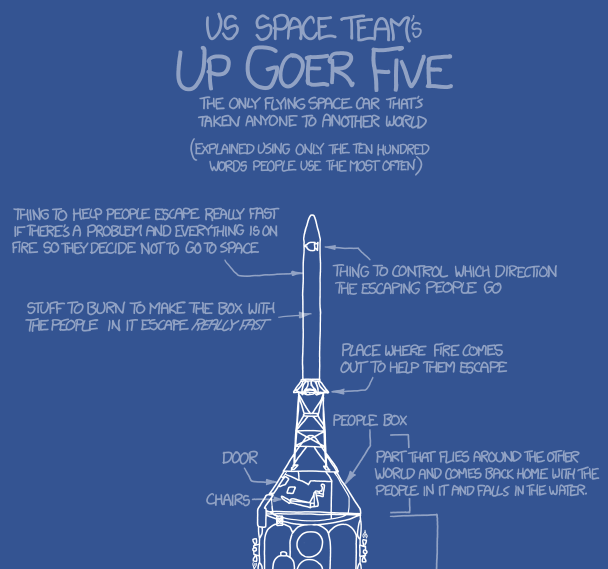
\includegraphics[width=\textheight]{Slides/Design/Daten/up_goer_five_part.png}
	\end{figure}
}

\frame{\frametitle{Einfache Sprache}
	\begin{itemize}
		\item angemessene Leseschwierigkeit
		\begin{itemize}
			\item Satzlänge
			\item Wortlänge
			\item Vokabular
				%jargon, acronyme, worthäufigkeitslisten
		\end{itemize}
		\item Sprache im Aktiv
		\item nur Schlüsselinformationen
	\end{itemize}
}
